\documentclass[a4paper,11pt,hidelinks]{scrartcl}

\usepackage[ngerman]{babel}
\usepackage{graphicx}
\usepackage{url}
\usepackage{listings}
\usepackage{fontspec}
    \setmainfont{Vollkorn}
    \setsansfont{Lato}
    \setmonofont{Inconsolata}

\renewcommand{\baselinestretch}{1.5}
\pagestyle{headings}

\newcommand{\imgref}[1]{{Abbildung \ref{#1}, Seite \pageref{#1}}}

\begin{document}

\author{Patrick Bucher}
\title{v13r g3w1nn7}
\subtitle{Gamedesign-Portfolio: Vier Gewinnt für Sysadmins}
\date{\today}
\maketitle
\thispagestyle{empty}

\begin{center}
    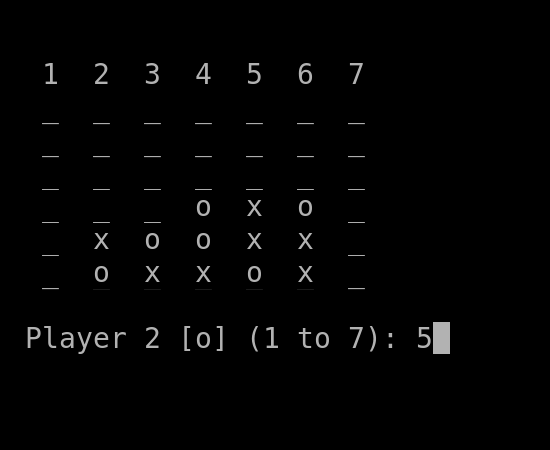
\includegraphics[width=0.5\linewidth]{pics/title.png}
\end{center}
%\newpage

\section*{Abstract}
Bla bla bla...
\newpage

\tableofcontents
\newpage

\section{Erste Iteration: Zieldefinition und Konzept}
\newpage

\section{Zweite Iteration: Anwendung von Game-Design-Theorie}
\newpage

\begin{figure}
    \centering
    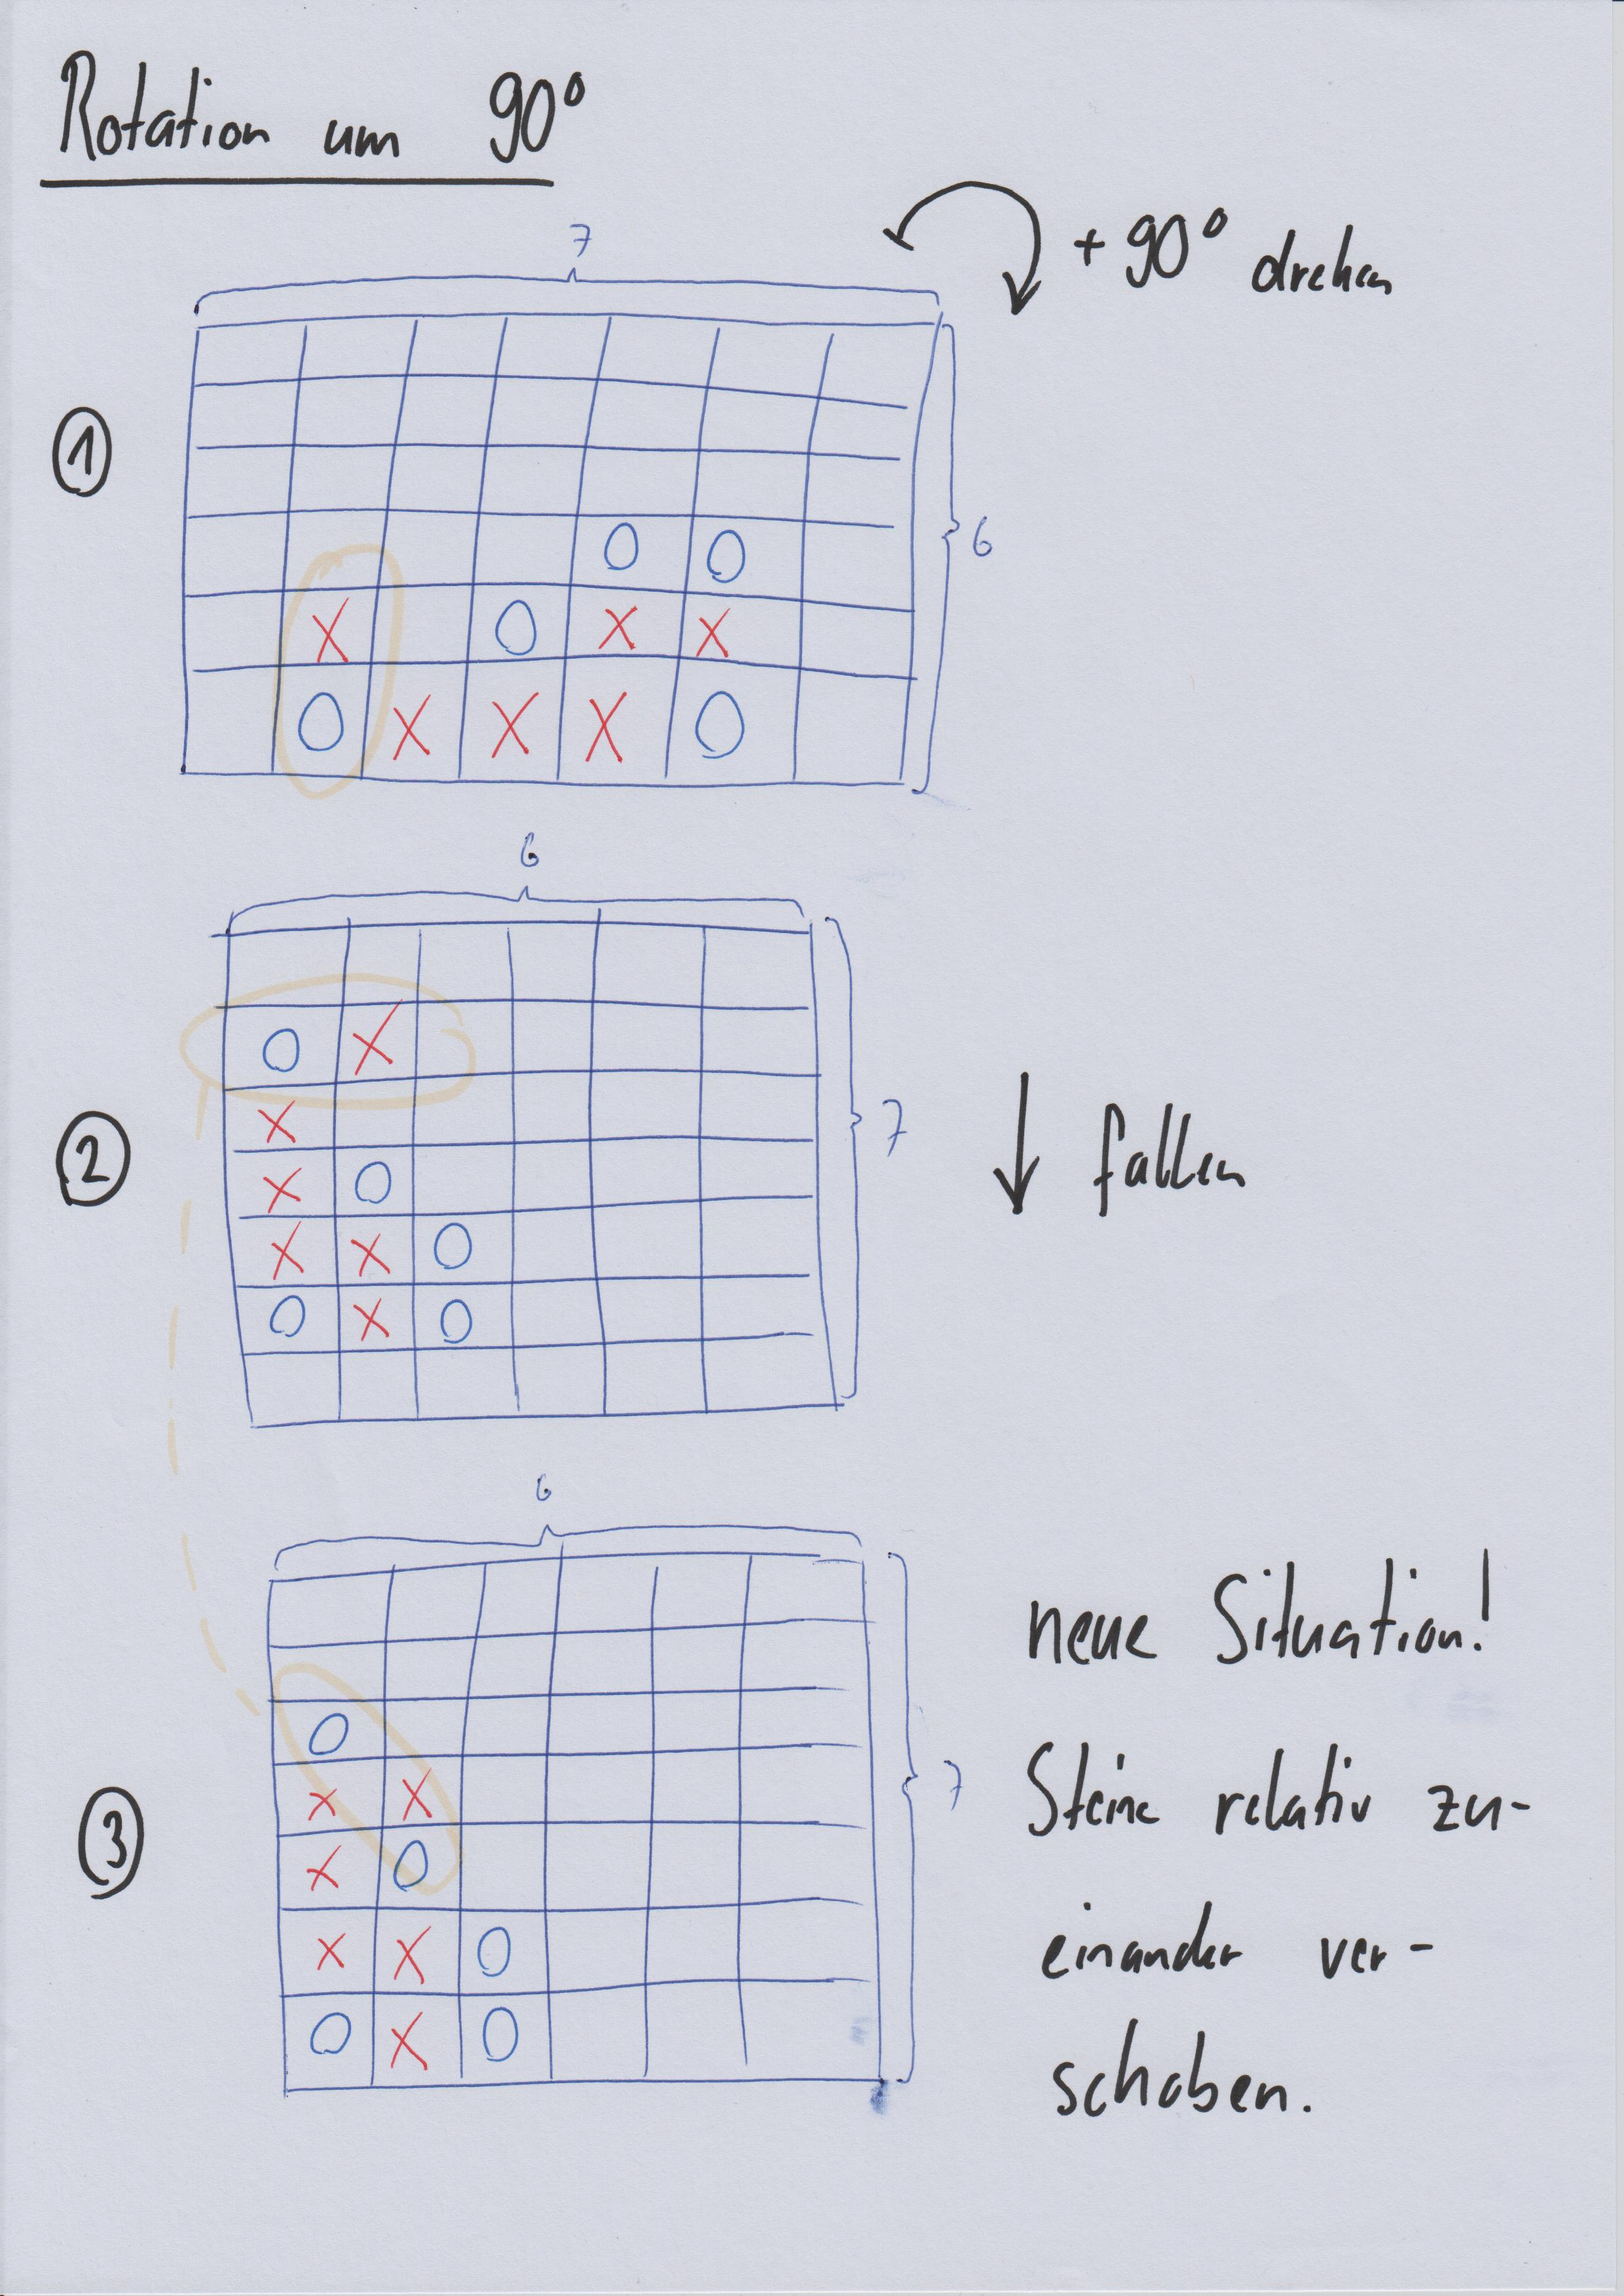
\includegraphics[width=0.7\linewidth]{pics/rotation-papier.jpg}
    \caption{Die Rotation um 90° als zusätzliche Spielmechanik. Das Spielgitter wird zunächst gedreht, anschliessend fallen die Steine nach unten. So entsteht eine neue Spielsituation, da sich manche Steine relativ zueinander bewegen.}
\end{figure}

\section{Dritte Iteration: Abschliessender Nutzertest und Reflexion}
\newpage

\listoffigures
\addcontentsline{toc}{section}{Abbildungsverzeichnis}

\end{document}
